\documentclass{article}
\usepackage[utf8]{inputenc}

\title{The Stock Market Today}
\author{Mike Medved, Benny Chen, Dan Paliulis}
\date{\today}

\usepackage{color}
\usepackage{amsthm}
\usepackage{amssymb} 
\usepackage{amsmath}
\usepackage{mathtools}
\usepackage{listings}
\usepackage[margin=1in]{geometry} 
\usepackage[dvipsnames]{xcolor}
\usepackage{tikz}

\newtheorem*{thm}{Theorem}

\begin{document}

\maketitle

\section{Introduction}

% introduction + background + objective statement

% how will the stock market react long-term to the pandemic, how is this different/similar vs 2008, what kind of techniques we can use this measure this.

The stock market is a very important part of the economy. It is a place where people can invest their money and make a profit. Many people rely on the stock market to make a living or to save up for retirement. There have been many crises throughout the history of the stock market. The stock market was first created in 1792 which helped many companies raise money to expand their businesses. One of the most famous crises in the stock market was the Great Depression. The Great Depression was a time period where the stock market crashed and many people lost their jobs. The Great Depression lasted from 1929 to 1939. After the Great Depression, many people found out how important the stock market was and how it effects the economy. After the Great Depression, the stock market has many ups and downs until the 2008 financial crisis. The 2008 financial crisis was again a time period where it repeated the Great Depression but it slowly recovered. The 2008 financial crisis was due to mainly the housing market at the time. The latest crisis that the stock market has faced is the COVID-19 pandemic. The COVID-19 pandemic has caused many companies to go  bankrupt and we are still feeling the effects of it to this day.

$\hfill \break$
In this paper, we will be talking about the effects of the COVID-19 pandemic and current situations today on the stock market. We will be using data from the Dow Jones Industrial Average (DJIA) from different points in time to see how the stock market reacts to different situations. Specifically, we will be looking at the Dow Jones Industrial (DJIA) Average from 2007 to 2009 and 2020 to today. From this data, we will be able to see how the stock market reacted from the pandemic and how it will react in the future.

\section{Data}

% what type of data we're processing, what we're doing with it programmatically, and where we're getting it from

% 2007 to 2009, 2020 to 2022
We are utilizing the below data from TradingView in order to guide our analysis, below we can see a candle graph of the prices of Dow Jones Industrial Average, as well as the Relative Strength Index (RSI) of it. Relative Strength Index (RSI) is a indicator that measures the magnitude and velocity of price changes. We are using this data to both predict the future of the stock market, as well as to see how the stock market has reacted to different crises.

$\hfill \break$
We chose the above time periods due to the extenuating circumstances occurring throughout them. In the case of 2007-2009, the dreaded 2008 economic collapse occurred, disrupting both the markets as a whole, and the Dow Jones Industrial Average as a result. We will also choose the time period of 2020 to today since we are still facing the effects of the COVID-19 pandemic to see how the stock market has reacted to it. Since we are still facing the consequences of the COVID-19 pandemic, we will be able to see how the stock market will be like in the future so we can better prepare ourselves for either growth or a decay.

\begin{figure}[!htb]
    \centering
    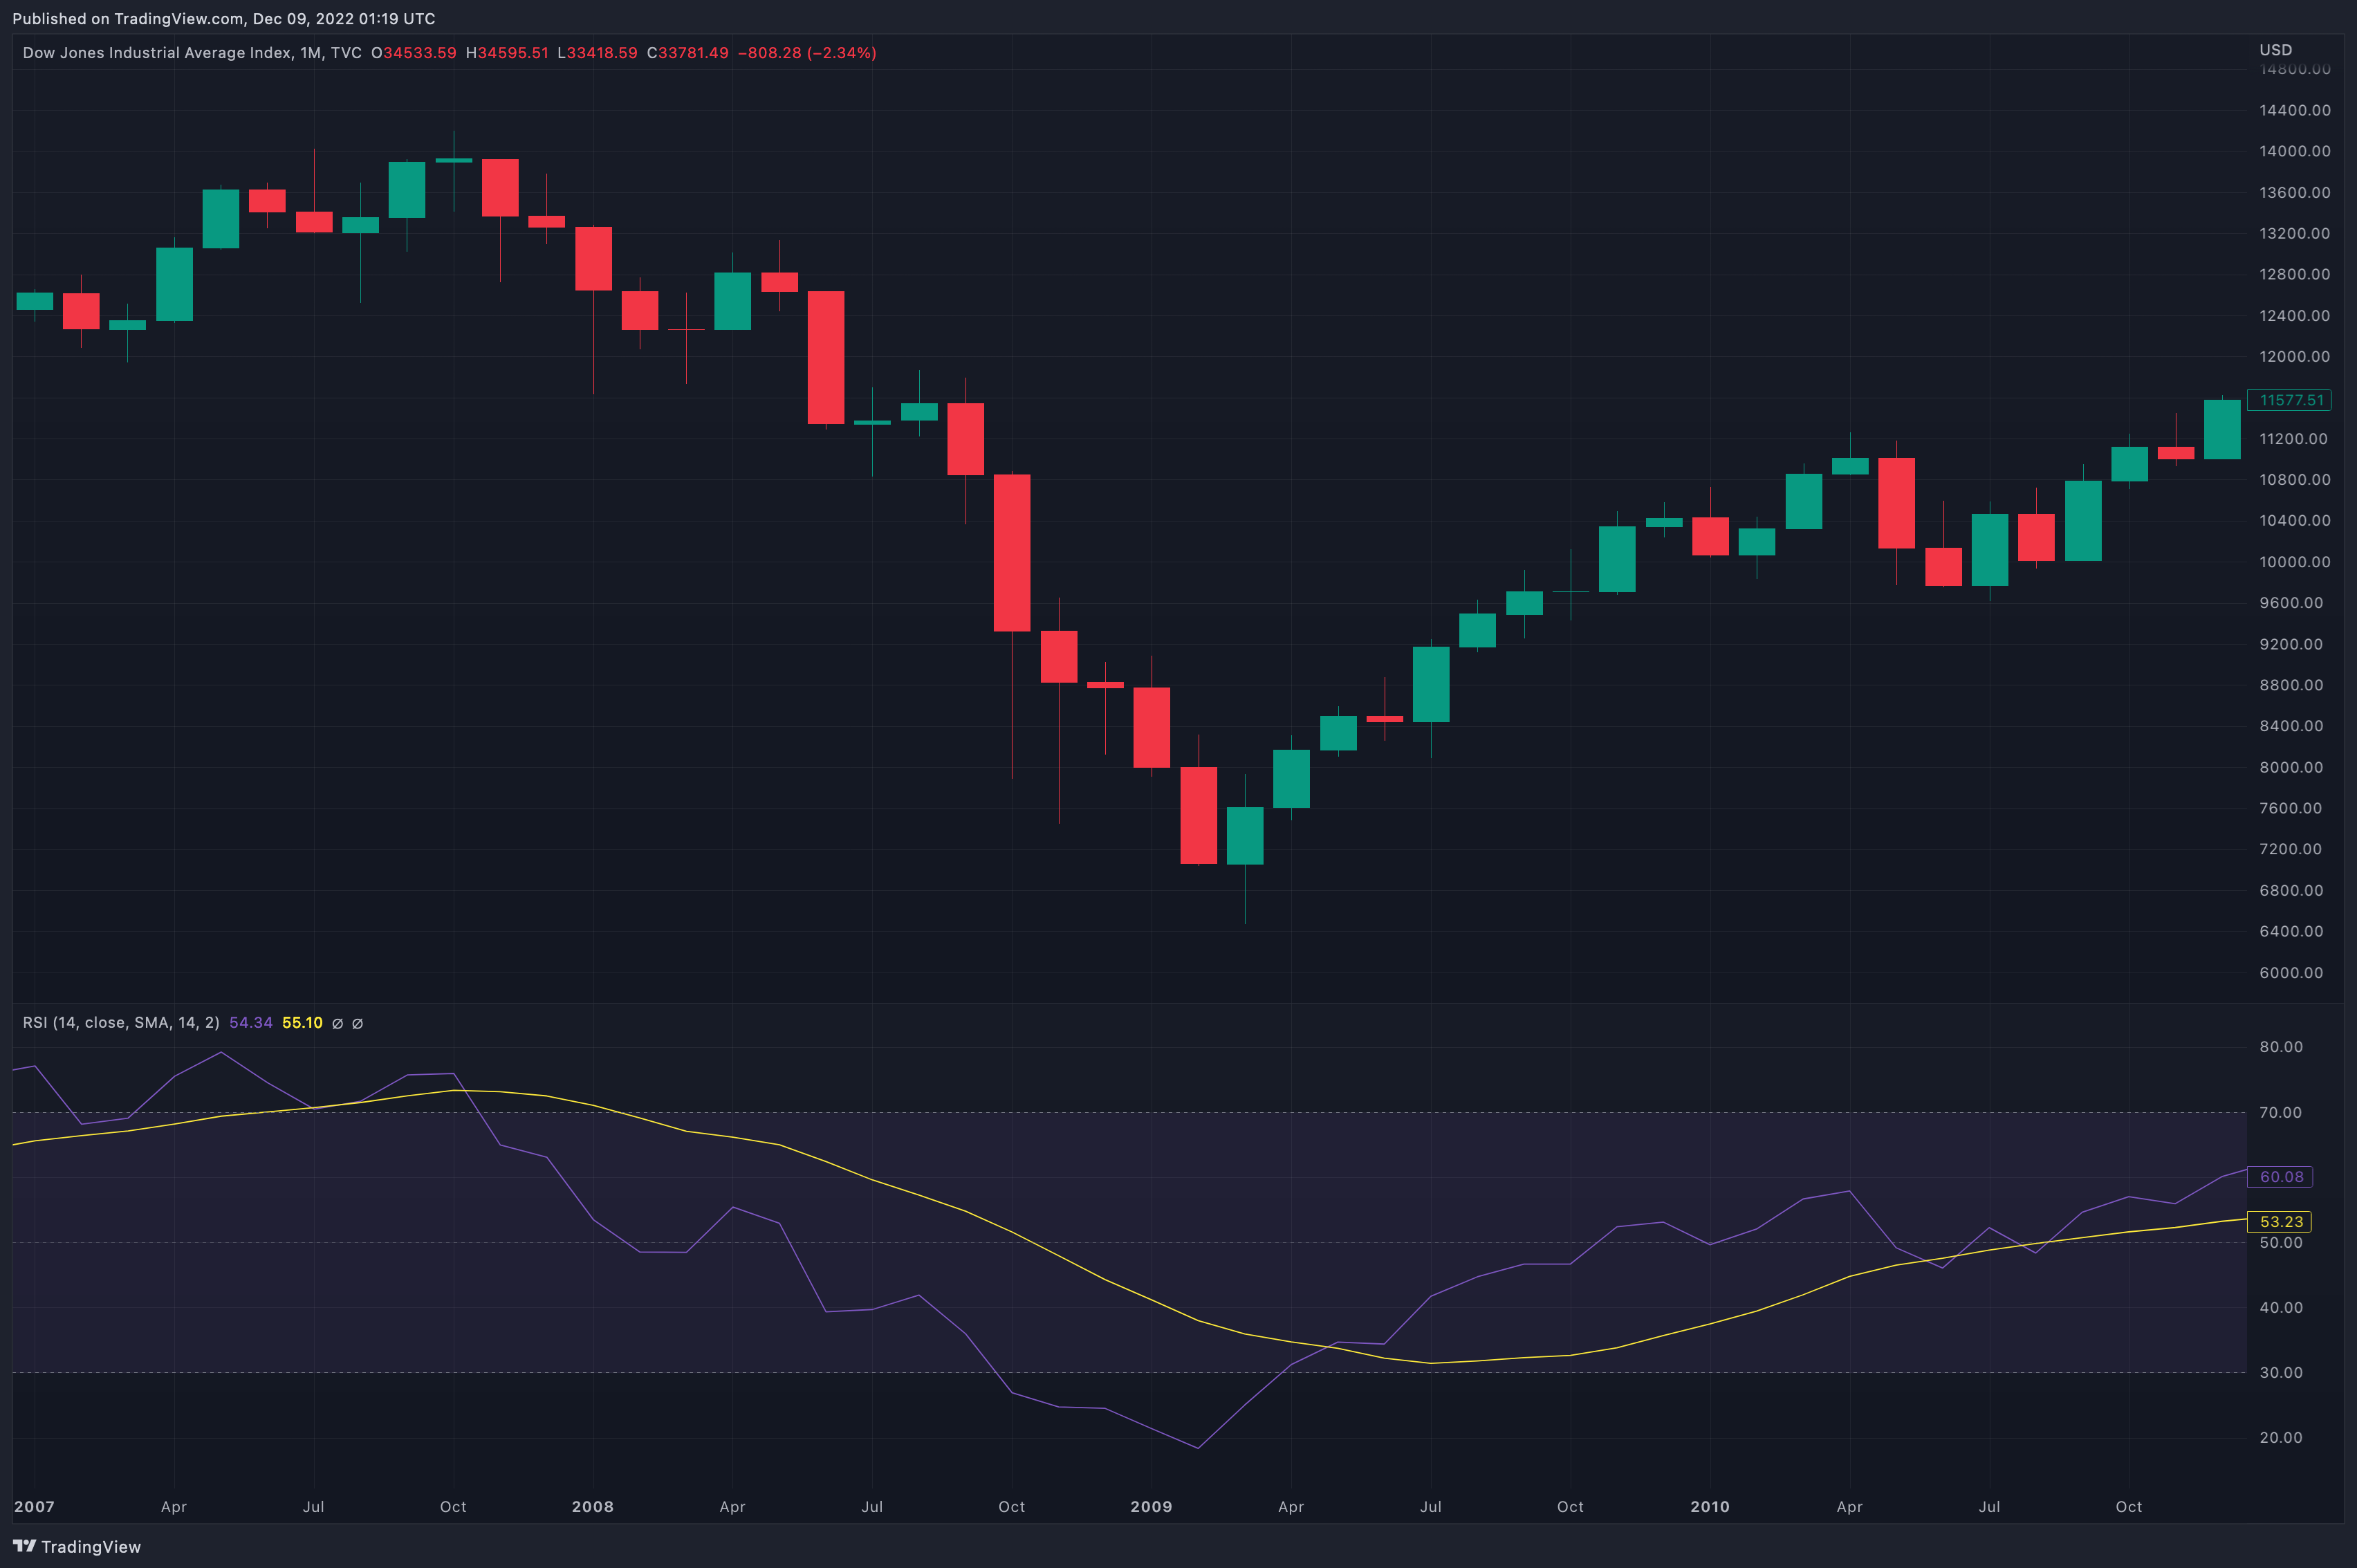
\includegraphics[scale=.125]{dow-2007-2010.png}
    \caption{Dow Jones Industrial Average (2007 to 2010)}
\end{figure}

\begin{figure}[!htb]
    \centering
    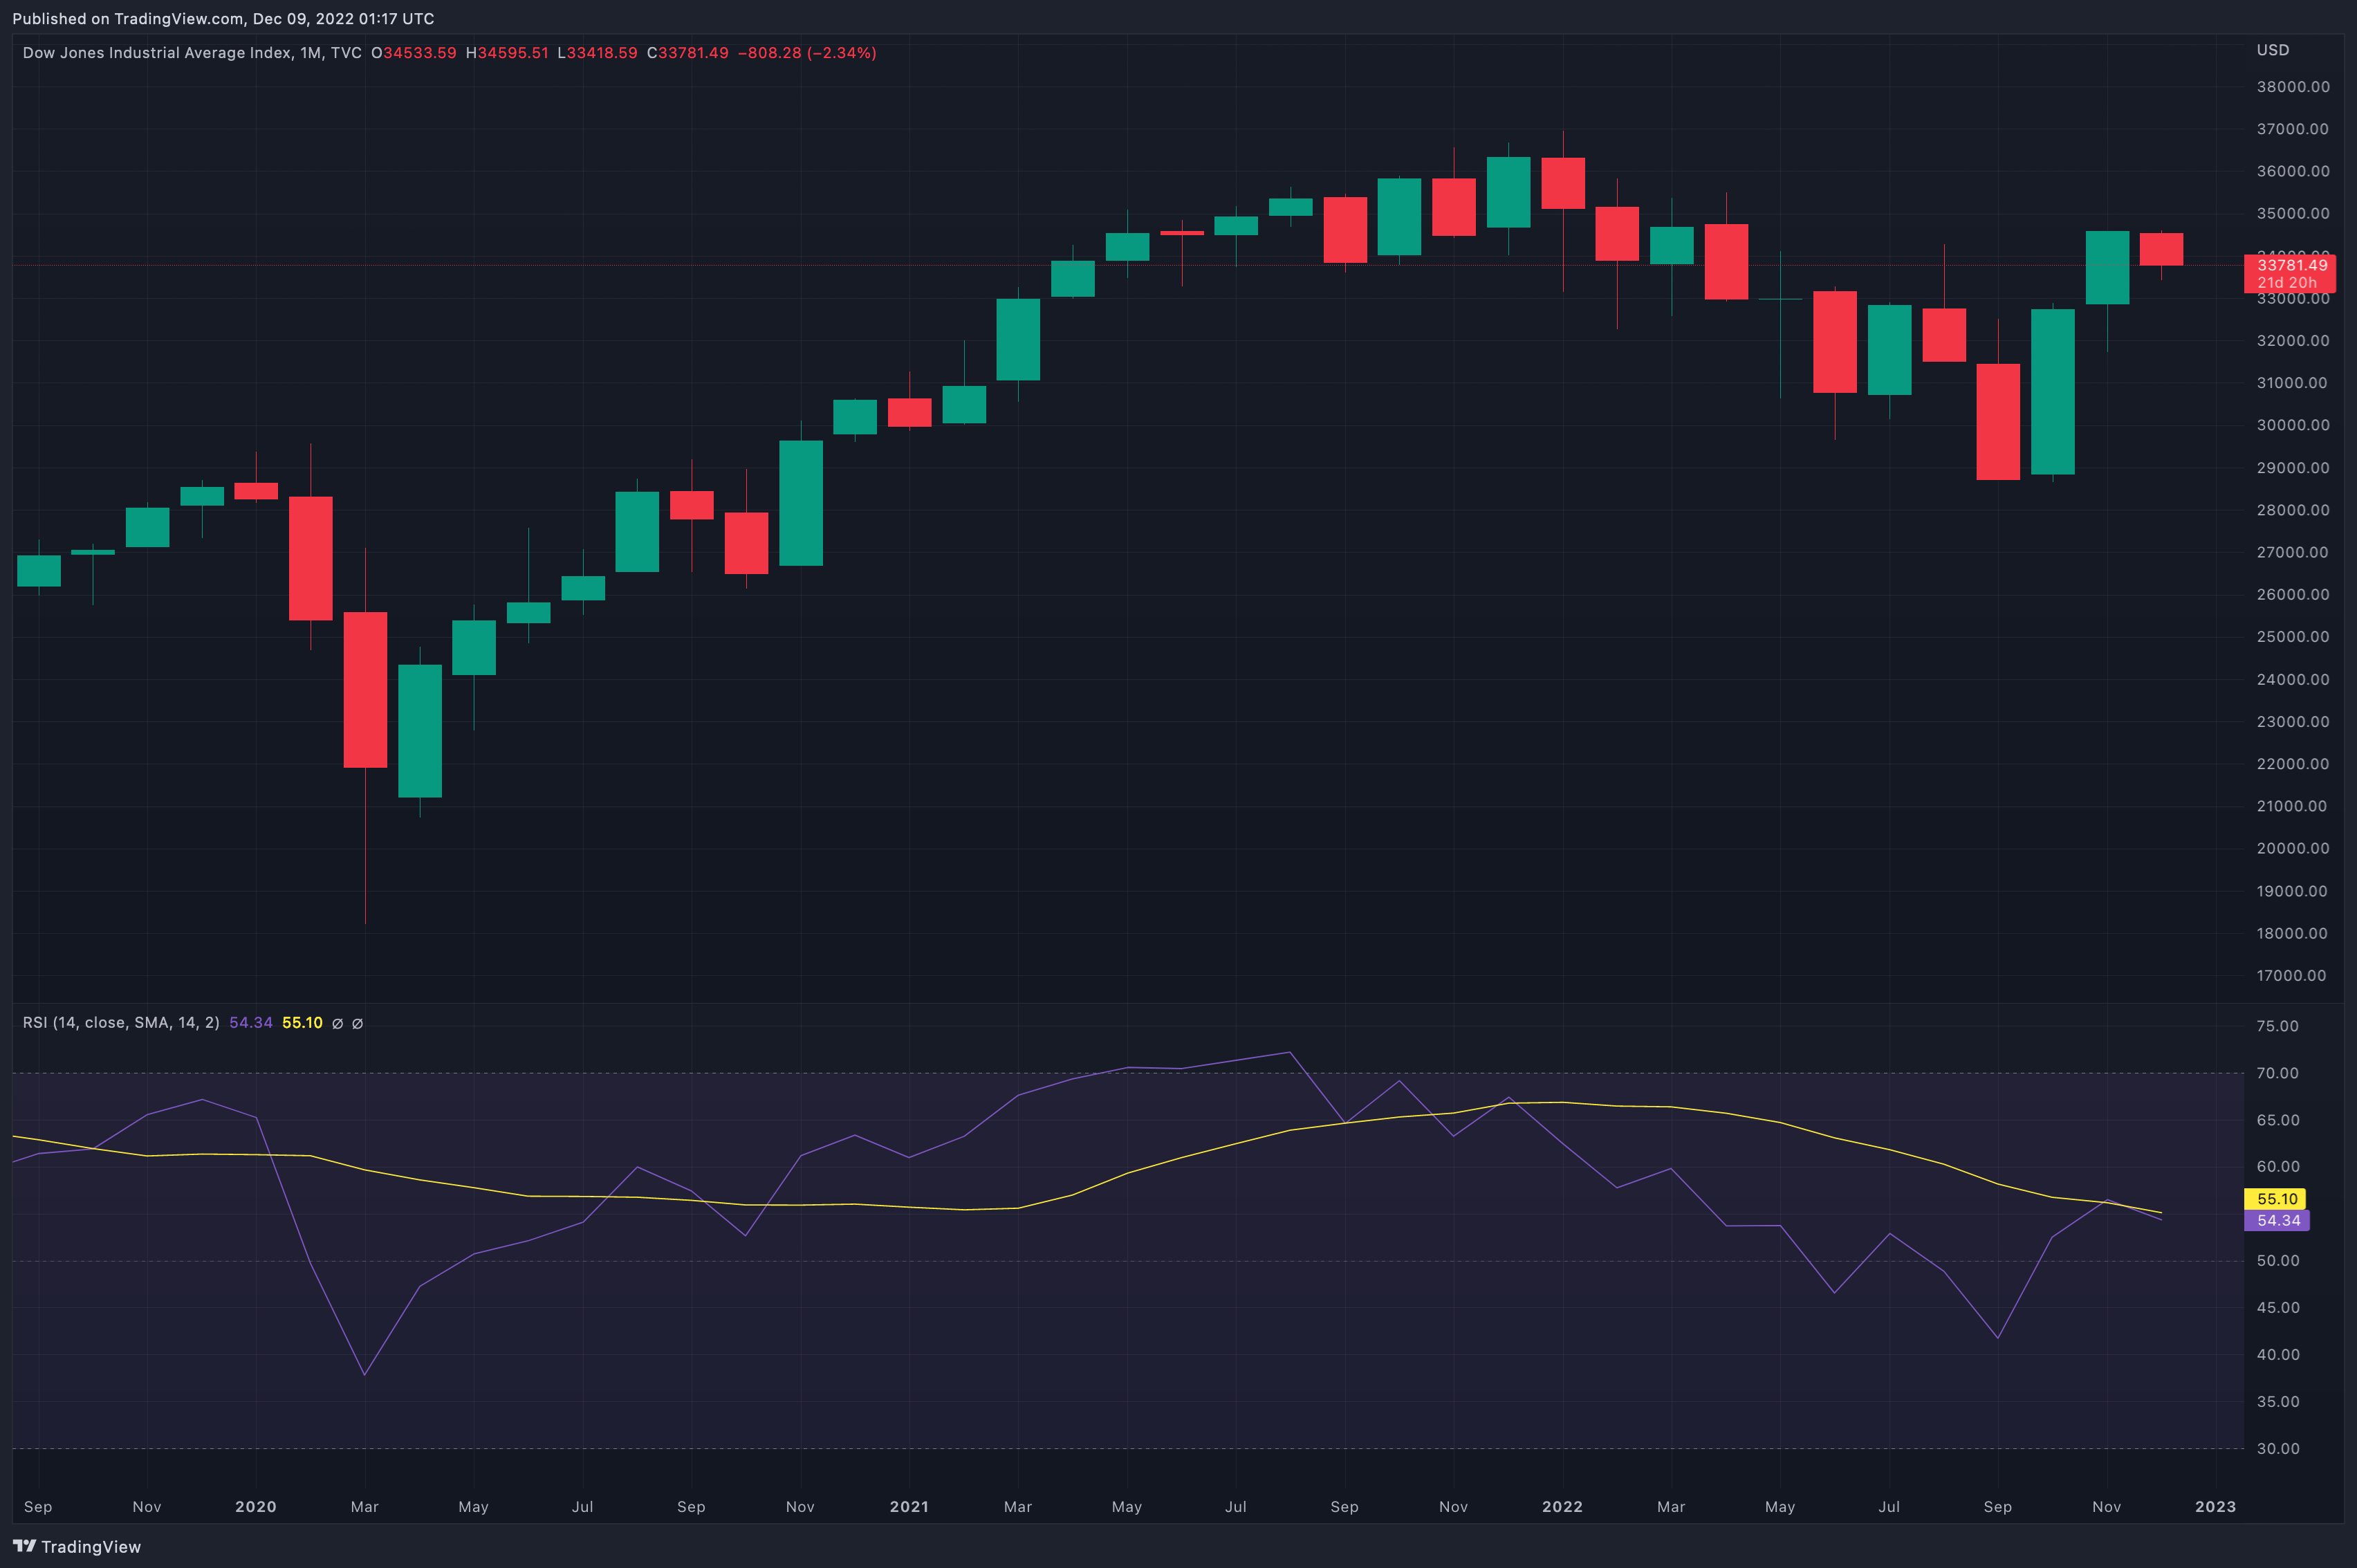
\includegraphics[scale=.125]{dow-2019-2022.png}
    \caption{Dow Jones Industrial Average (2019 to 2022)}
\end{figure}

\newpage

\section{Analysis}

% analysis of data & math, give charts and some insights to said charts
According to the above graphs, we can clearly see a cohesive picture of how external sentiment can affect the stock market as a whole. This is because the Dow Jones Industrial Average represents a significant portion of global stock trades, and when it recedes, it indicates a larger economic event.

$\hfill \break$
In this way, we can observe the cataclysmic affect of COVID-19 on the global economic forecast through the sharp decline in both the Relative Strength Index (RSI) and the nominal value of the Dow. Interestingly, we can see how these events influence the Volatility Index (VIX) and furthermore how these events inflict damage on society through the rapid inflation that is generally associated with them.

\begin{figure}[h]
    \centering
    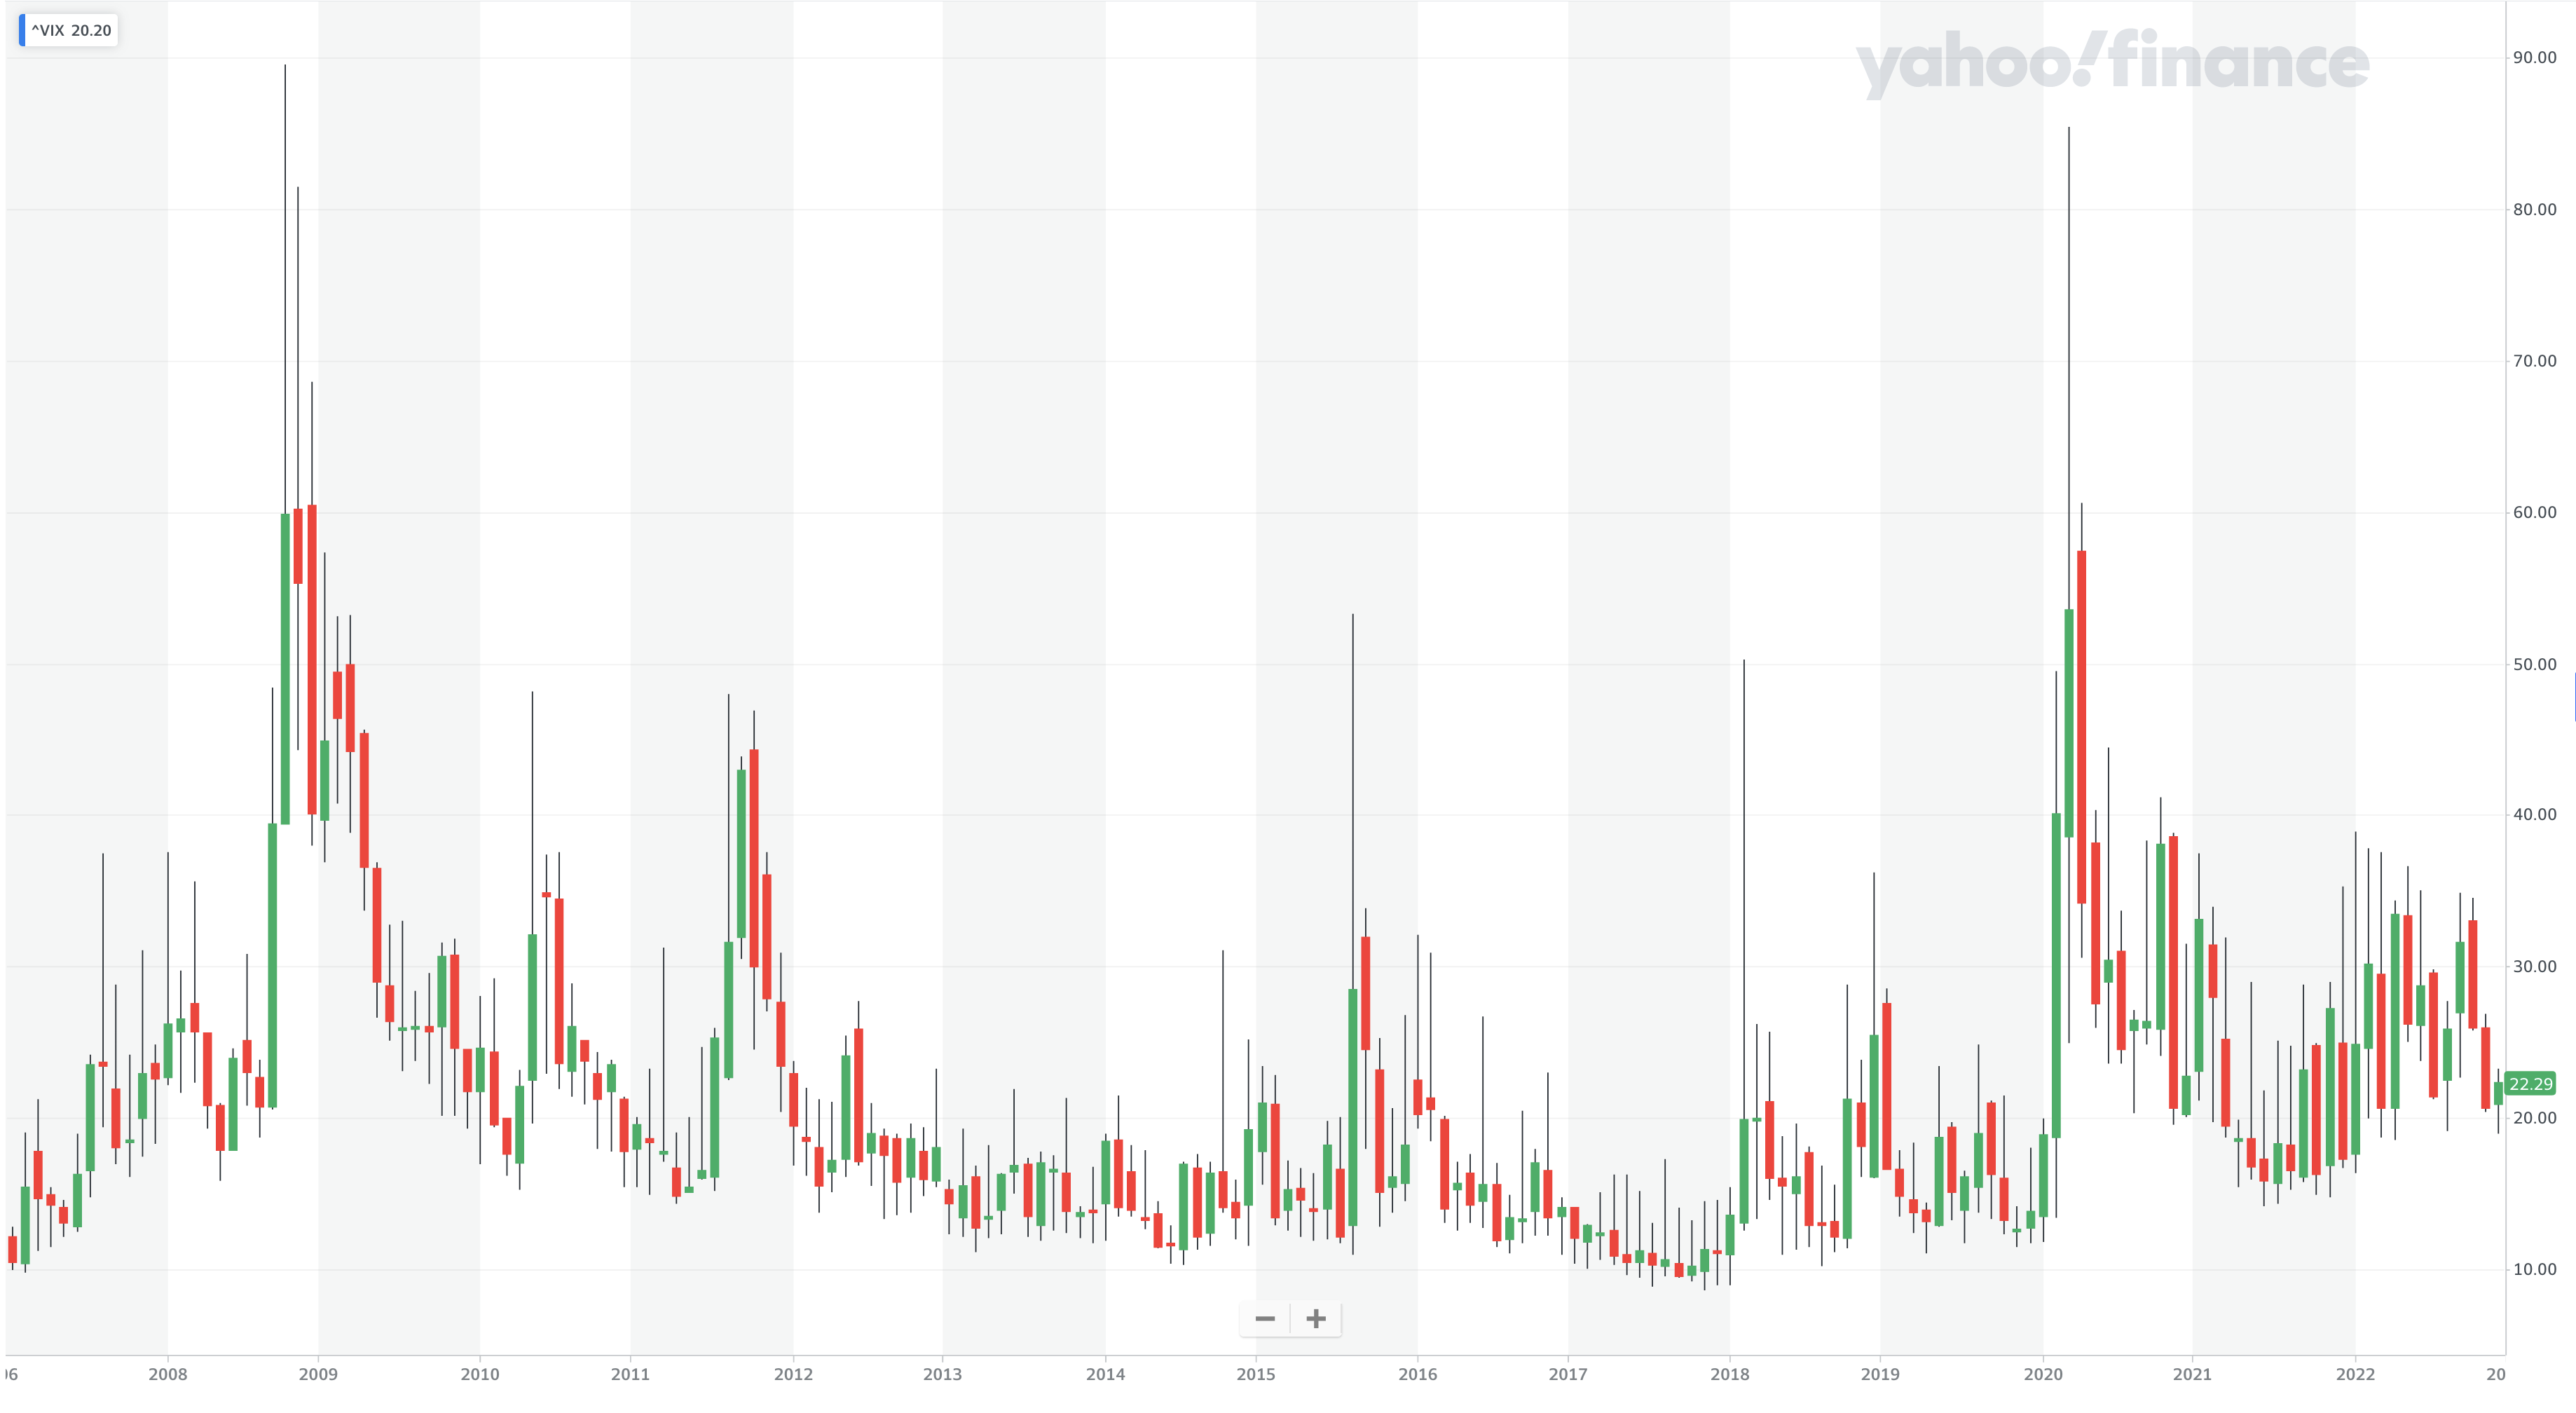
\includegraphics[scale=0.25]{vix-2007-2022.png}
    \caption{Volatility Index (2007 to 2022)}
\end{figure}

\section{Theory}

% how do we form continuous random variables from the discrete datasets (s&p 500, nasdaq, dow, vix, etc.) and how are these used to compute finite probabilities that reflect future sentiment with respect to the market(s).

In these graphs, we are displaying the stock market trend data from January 2007 to December 2010, and data from September 2019 to December 2022 of the Dow Jones Industrial Average. We chose these dates to show how the stock market trends dipped due to 
the economic recession of 2008 and the Coronavirus pandemic of 2020. We are also displaying the relative strength index of the graphs. The Relative Strength Index (RSI) is a momentum indicator measuring the speed and magnitude of price changes.

$\hfill \break$
The relative strength index is a number on the interval [0, 100] calculated as follows:
$$
\text{RSI = }100 - \frac{100}{1 + RS}
$$

$\hfill \break$
where $RS$ represents the relative strength, calculated by analyzing the average gains and losses over a period of time.

$\hfill \break$
This allows us to predict the price behavior of a stock by indicating how quickly it's price will increase or decrease based on how quickly traders bid the price. Given that a relative strength is calculated from an average of values, we can use
the central limit theorem to find the probability that the relative strength will lie above a particular constant value. There are two definitions to define the central limit theorem. Version 1 states that, given random variables
$X_1, ..., X_n$, we have that their average can be approximated as a general normal random variable. This theorem requires that all random variables $X_1, ..., X_n$ are independent and identically distributed, meaning that any two random variables in 
$X_1, ..., X_n$ do not affect each other's probability, and that all random variable $X_1, ..., X_n$ are of the same type. We also have that any random variable $X_k$ from $X_1, ..., X_n$ has the expectation $\mu$ and the variance $\sigma^2$. We can show this formulaically
as 
$$
\frac{X_{1} + ... + X_{n}}{n} \approxeq \mathcal{N}\left(\mu, \frac{0}{1}\right)
$$
Note that this definition holds for large values of n. We write version 2 of the central limit theorem using the standard normal random variable. This is defined as follows:
$$
\lim_{n \to \infty}\frac{\frac{X_{1} + ... + X_{n}}{n} - \mu}{\frac{\sigma}{\sqrt{n}}} \approxeq \mathcal{N}\left(\mu, \frac{\sigma^2}{n}\right)
$$
Note that here we are taking advantage of the reduction to standard normal, which goes as follows:
$$
\text{Given } X \sim \mathcal{N}\left(\mu, \sigma^2\right)\text{, we have }
\frac{X - \mu}{\sigma}\sim \mathcal{N}\left(0, 1\right)
$$
Therefore, we can calculate that the relative strength lies above a constant value with the following reduction. Let $X_k$ be the gains and losses at a time k, where we have random Variables
$X_1, ..., X_n$, with n = t - $t_0$. Let $\mu$ be the equivalence of each individual random variable, and $\alpha^2$ be the variance of each individual random variable. Additionally, let $\alpha$ = n * $\beta$, were we are trying to find the probability that the relative strength is greater than the constant $\beta, P(RS > \beta)$. We have the following:

\begin{align*}
P(X_1, ..., X_n > \alpha) &= P\left(\frac{X_1 + ... + X_n}{n} > \frac{\alpha}{n}\right) \\
&= P\left(\frac{X_1 + ... + X_n}{n} - \mu > \frac{\alpha}{n} - \mu\right) \\
&= P\left(\frac{\frac{X_1 + ... + X_n}{n} - \mu}{\sigma} > \frac{\frac{\alpha}{n} - \mu}{\sigma}\right) \\
&= P\left(Z > \frac{\frac{\alpha}{n} - \mu}{\sigma}\right)\text{ where Z } \sim \mathcal{N}(0, 1) \\
&= 1 - P\left(Z < \frac{\frac{\alpha}{n} - \mu}{\sigma}\right) \\
&= 1 - \phi\left(\frac{\frac{\alpha}{n} - \mu}{\sigma}\right) \\
\end{align*}
$\hfill \break$
We can use what we have shown in our problem statement to predict stock market trend fluctuations using continuous random variables. 
We would do this by using the central limit theorem to calculate the probability that the relative strength will be above a certain value.
With this, we can make decisions on how probable specific relative strength indices are at a future time.


\section{Lasting Impact}

The stock market is an ever-changing entity, and we are currently in the midst of a major shift in the global economy. With the rise of cryptocurrency, new financial instruments, and spiking volatility, right now is one of the most pivotal times in the market, and we are observing it adapting with new listings, investment strategies, and the rise of super-advanced quant trading.

\begin{thebibliography}{3}
    \bibitem{https://www.investopedia.com}
    https://www.investopedia.com

    \bibitem{https://www.tradingview.com}
    https://www.tradingview.com

    \bibitem{https://finance.yahoo.com}
    https://finance.yahoo.com

\end{thebibliography}

\end{document}